\chapter{Разработка модели идентификации имплантируемого роторного насоса крови и математической модели сердечно-сосудистой системы} \label{chapt2}

Цель данной главы заключается в разработке модели идентификации имплантируемого роторного насоса крови и математической модели сердечно-сосудистой системы с учетом имплантации роторного насоса крови.  

%а основе расходно-напорных характеристик (РНХ), полученных в результате экспериментального исследования имплантируемых роторных насосов крови и опубликованных в литературе.

\section{Анализ исходных данных}

В качестве исходных экспериментальных данных выбраны расходно-напорные характеристики (РНХ) имплантируемого роторного насоса крови HeartMate II, опубликованные в работах \cite{Pennings_2013, Stanfield_2012} и представленные на рисунке \ref{img:initial_data}.

\begin{figure}[ht]
  \begin{minipage}[ht]{0.48\linewidth}
    \center{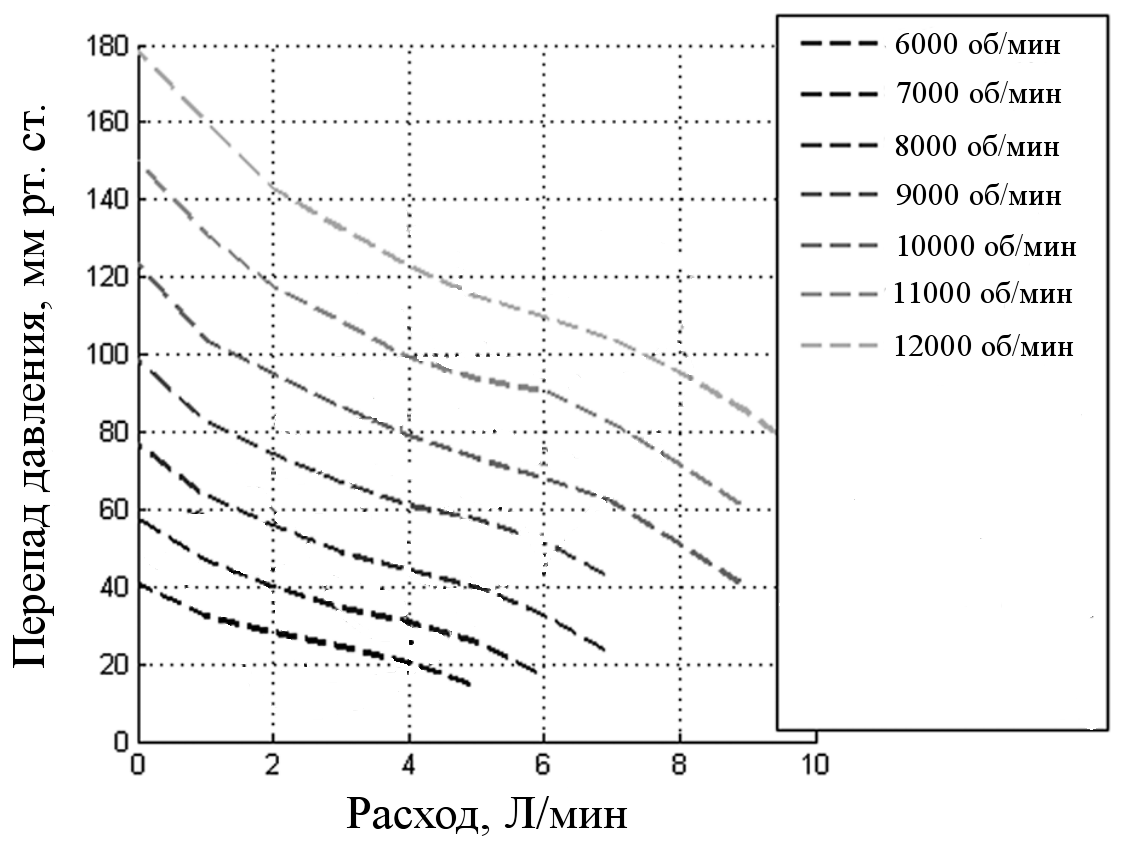
\includegraphics [scale=0.35] {../images/c2_basic_hq_static} \\ а)}
  \end{minipage}
  \hfill
  \begin{minipage}[ht]{0.48\linewidth}
    \center{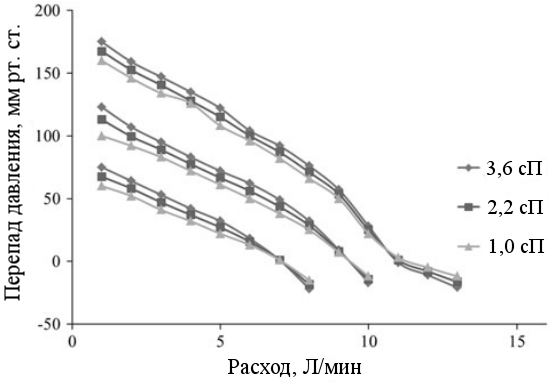
\includegraphics [scale=0.43] {../images/c2_basic_hq_static_viscosity} \\ б)}
  \end{minipage}
  \caption{Расходно-напорные характеристики имплантируемого роторного насоса крови HeartMate II из работы Pennings и др. \cite{Pennings_2013} и Stanfield и др. \cite{Stanfield_2012}}
  \label{img:initial_data}  
\end{figure}

Влияние вязкости жидкости, перекачиваемой насосом при различных величинах скорости вращения ротора, показано на рисунке \ref{img:initial_data}б. Так, изменение вязкости от 3,6 до 1,0 сП приводит к изменению наклона рассматриваемой характеристики. В случае уменьшения вязкости до 1,0 сП при фиксированном перепаде давления (например, 100 мм рт. ст.) происходит уменьшение расхода примерно на 1-1,2 л/мин. С уменьшением перепада давления влияние вязкости уменьшается, однако при отрицательном перепаде давлений влияние вязкости крови прямо противоположно: ее уменьшение приводит к увеличению расхода при фиксированном перепада давления. 

Необходимость учета влияния вязкости жидкости при разработке математических моделей имплантируемых роторных насосов крови обосновывается в работах \cite{Malagutti_2007, Pennings_2013, 4352467}. О необходимости учета влияния вязкости жидкости был сделан доклад на конференции <<МедТех>> \cite{medtech_2014}.

В ходе анализа ранее опубликованных работ \cite{Moscato_2009, Pirbodaghi_2011} для описания РНХ имплантируемого роторного насоса крови было выбрано следующее уравнение:

\begin{equation}
	\label{eq:initial_eq}
	L\frac{dQ}{dt} = (a_1\mu+a_2)Q + (b_1\mu+b_2)\omega^2 + H,
\end{equation}

\noindent где $L$ -- параметр, характеризующий инерцию жидкости в данном насосе (мм рт. ст.$~\cdot$ мин$^2~\cdot$ л$^{-1}$) \cite{Moscato_2009}, $Q$ -- расход насоса (л/мин), $\mu$ -- параметр, характеризующий вязкость жидкости в насосе (сП), $\omega$ -- скорость вращения ротора насоса (об/мин), $H$ -- перепад давления в насосе (мм рт. ст.), $a$ и $b$ -- коэффициенты, представленные линейной функцией вида $x(\mu) = x_1\mu + x_2$, что позволяет учесть изменение в наклоне расходно-напорной характеристики при изменении вязкости жидкости ($\mu$, сП) \cite{Malagutti_2007}. 

Параметр $L$ выбран равным 0,2, значения коэффициентов уравнения \eqref{eq:initial_eq} определены с помощью процедуры оптимизации, описание которой приводится далее. Оптимизация коэффициентов уравнения проведена по точкам, которые были выбраны в ходе анализа расходно-напорных характеристик роторного насоса крови HeartMate II и отмечены круглыми маркерами на рисунке \ref{img:pump_identification_first_stage}.

Расходно-напорные характеристики, описываемые уравнением \eqref{eq:initial_eq}, представлены на рисунке \ref{img:pump_identification_first_stage}. 

% Так, параметр $L$ выбран произвольно и, согласно работе \cite{Moscato_2009}, для реального насоса он может быть другим. Влияние вязкости воспроизведено также примерно, хотя та динамика РНХ, которая наблюдается на экспериментальных кривых, повторяется моделью совершенно точно. 

\section[Процедура оптимизации]{Процедура оптимизации коэффициентов модели идентификации}

В ходе исследования была разработана процедура оптимизации коэффициентов математической модели идентификации на основе алгоритма Левенберга-Марквардта \cite{IMM2004, gavin2011levenberg}, которая позволяет обеспечить соответствие между выходными данными математической модели и набором искомых значений или экспериментальных данных. 

Основная задача алгоритма заключается в оптимизации вектора параметров $\beta$ целевой функции $f(x, \beta)$ относительно эмпирических значений $y$ таким образом, чтобы сумма вектора невязки $S(\beta)$ была минимальной:

\begin{equation}
	S(\beta) = \sum_{i=1}^{m} [y_i - f(x_i, \beta)]^2
\end{equation}

В качестве параметра $x$ целевой функции $f$ задан массив \verb!p1!, в качестве параметра $\beta$ -- массив \verb!v_i!. 

Подобно другим численным алгоритмам оптимизации, данный алгоритм является итерационной процедурой. Первоначально формируется начальное приближение для вектора параметров $\beta$. Предполагается, что для случая с только одним минимумом хорошо работает приближение вида $\beta = (1,0, 1,0, \ldots, 1,0)$.

На каждой итерации находится приращение $\delta$ к вектору параметров $\beta$. Основное уравнение алгоритма Левенберга-Марквардта выглядит следующим образом:

\begin{equation}
	(J^T J + \lambda ~diag(J^TJ))\delta = J^T[y-f(\beta)]
	\label{eq:lm_method}
\end{equation}

\noindent где $J$ -- матрица Якоби, $J^T$ -- транспонированная матрица Якоби, $\lambda$ -- коэффициент затухания, $\delta$ -- искомое приращение к вектору параметров $\beta$, $y$ -- искомые значения, $f$ -- целевая функция.

%В уравнении \eqref{eq:lm_method} используется диагональная матрица, содержащая диагональные элементы $J^TJ$. %, которая в данной работе в большинстве случаев заменена на матрицу идентичности $I$, т.\:е. используется версия алгоритма без модификации Марквардта. 

Значение каждого элемента матрицы Якоби описывается следующим уравнением: 

\begin{equation}
	J_i = \frac{\partial f(x_i, \beta)}{\partial \beta}
\end{equation}

Исходное неотрицательное значение коэффициента затухания $\lambda$ установлено эмпирически. Значение коэффициента может быть изменено на каждой итерации. Например, в случае быстрого уменьшения суммы вектора невязки значение коэффициента может быть уменьшено. 

Матрица Якоби вычисляется как разность между векторами невязок \verb!r! и \verb!rr!. Вектор невязки \verb!r! вычисляется как разность между массивом значений целевой функции \verb!M!, полученных с использованием вектора параметров \verb!p_i!, и массивом искомых значений \verb!T!. Вектор невязки \verb!rr! вычисляется с использованием вектора параметров \verb!pp_i!, полученных в результате отклонения массива \verb!v_i! на шаг \verb!dx!. 

Для перемножения матриц используется функция \verb!dot! из библиотеки NumPy, для нахождения приращения \verb!s! -- функция \verb!lstsq! из библиотеки NumPy.

Целевая функция может быть критична к выбору параметров \verb!v_i!, например, они должны быть неотрицательны. Чтобы учесть это были введены проверки на величину приращений \verb!s!: если оно больше, чем значение соответствующего параметра \verb!v_i!, то оно делится на десять -- данное значение подобрано эмпирически и может быть любым. 

Процедура оптимизация реализована на языке программирования Python с использованием библиотеки NumPy. Программный код приведен в приложении \ref{list:optimization_routine}. При разработке использованы результаты диссертационной работы W. Smith <<Minimal heamodynamic modelling of the heart \& circulation for clinical applications>>.

\section{Алгоритм структурно-параметрической идентификации}

В ходе анализа полученных результатов было установлено несоответствие между формой моделируемых расходно-напорных характеристик, представленных на рисунке \ref{img:pump_identification_first_stage}, и формой исходных РНХ, представленных на рисунке \ref{img:initial_data}. 

\begin{figure}[ht]
  \center{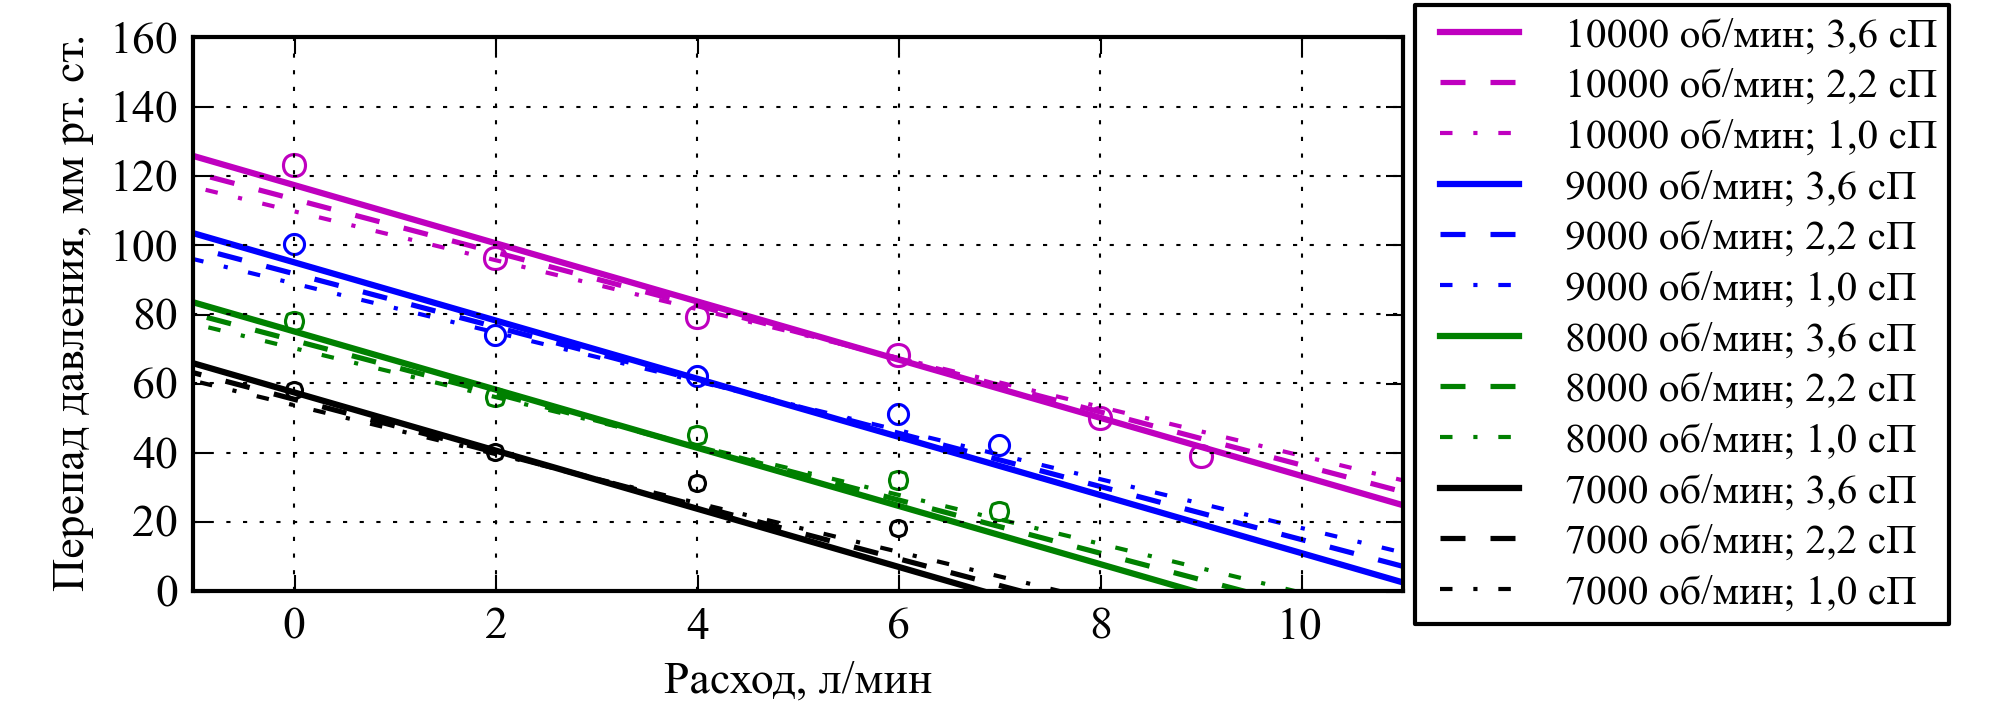
\includegraphics [scale=0.99] {../images/c2_static_model_initial_dis}}
  \caption{Расходно-напорные характеристики роторного насоса крови, описываемые уравнением \eqref{eq:initial_eq}}
  \label{img:pump_identification_first_stage}  
\end{figure}

Решением данной проблемы стала разработка алгоритма структурно-параметрической идентификации. Основная идея алгоритма заключается в последовательном добавлении одночленов $kx_j$ к исходному уравнению $y_i$ и отборе уравнений вида $y_i + kx_j$ посредством сравнения с критерием оценки эффективности идентификации на каждой итерации алгоритма $i$. 

Схема алгоритма идентификации представлена на рисунке \ref{img:flowchart}.

\begin{figure}[!ht]
\centering
\begin{tikzpicture}[node distance=1cm, auto]  

\tikzstyle{startstop} = [rectangle, rounded corners=10pt, minimum width=3.0cm, minimum height=1.35cm,text centered, draw=black]
\tikzstyle{io} = [trapezium, trapezium left angle=70, trapezium right angle=110, minimum width=0.9cm, minimum height=1.1cm, text centered, draw=black]
\tikzstyle{process} = [rectangle, minimum width=1.1cm, minimum height=1.3cm, text centered, draw=black]
\tikzstyle{decision} = [diamond, minimum width=3.1cm, minimum height=1.35cm, text centered, draw=black]
\tikzstyle{arrow} = [thick,->,>=stealth]

\node (s) [startstop, yshift=-20.0, minimum height=0.9cm] {\parbox{4.5cm}{\small \centering Начало}};
\node (start) [process, below of=s, yshift=-20.0] {\parbox{5.95cm}{\small Задание исходного уравнения $y_i$ где $i$ -- номер итерации }};
\node (in1) [io, below of=start, yshift=-1.05cm] {\parbox{5.55cm}{\small Добавление к $y_i$ одночлена $kx_j$ где $k$ -- коэффициент \\ $j$ -- номер одночлена}};
\node (pro1) [process, below of=in1, yshift=-1.50cm] {\parbox{7.80cm}{\small Определение коэффициентов $y_i + kx_j$ с \\использованием процедуры оптимизации \\ Проверка соответствия критерию оценки эффективности идентификации}};
\node (dec1) [decision, below of=pro1, yshift=-1.30cm] {};% {\footnotesize\bf \parbox{1.5cm}{Соответствие \\ критериям}};
\node (dec2) [decision, below of=dec1, yshift=-0.75cm] {};
\node (out2a) [process, right of=dec2, yshift=0.0cm, xshift=5.2cm, minimum width=1.0cm] {\parbox{4.15cm}{\small Задание $y_i + kx_j$ \\исходным уравнением \\ $i = i + 1$ \\ $j = j + 1$}};
\node (out2b) [io, left of=dec1, xshift=-5.3cm, minimum width=1.0cm] {\parbox{3.70cm}{\small Исключение $y_i + kx_j$ \\ $j = j + 1$}};
\node (out2c) [process, below of=dec2, yshift=-0.8cm, minimum height=1.0cm] {\small Окончательное $y_i + kx_j$};
\node (out) [startstop, below of=out2c, yshift=-0.5cm, minimum height=0.9cm] {\parbox{4.5cm}{\small \centering Конец}};

\draw [arrow] (s) -- (start);
\draw [arrow] (start) -- (in1);
\draw [arrow] (in1) -- (pro1);
\draw [arrow] (pro1) -- (dec1);
\draw [arrow] (out2c) -- (out);
\draw [arrow] (dec2) -- node[anchor=south] {\small нет} (out2a);
\draw [arrow] (dec1) -- node[anchor=south] {\small нет} (out2b);
\draw [arrow] (dec1) -- node[anchor=west] {\small ~да} (dec2);
\draw [arrow] (dec2) -- node[anchor=west] {\small ~да} (out2c);
\draw [arrow] (out2a) |- ($(in1.east)+(0,-0.1)$);
\draw [arrow] (out2b) |- ($(in1.west)+(0.05,0.1)$);
%\draw [arrow] (out2b) ($(out2b.east)$)|- + (2.5,0) |- ($(in1.east)+(0.05,0.1)$); 
\draw (0.0, -9.33) node {\small $R^2_{ij} > R^2_i$}; %  \\ $\delta(PS) \geq 85\%$
\draw (0.0, -11.05) node {\small $R^2_{ij} \geq 0,9980$}; %  \\ $\delta(PS) \geq 85\%$
\end{tikzpicture} 
\caption{Схема алгоритма идентификации роторного насоса крови} 
\label{img:flowchart}  
\end{figure}

%Работа алгоритма завершается в случае соответствия требуемой величине $R^2$.

В качестве исходного уравнения $y_i$ было выбрано уравнение \eqref{eq:initial_eq}. Список одночленов $kx_j$ был сформирован в результате анализа математических моделей роторных насосов крови, описанных в литературе и рассмотренных в разделе \ref{identification_review}. Каждый одночлен представляет собой произведение коэффициента $k$ и переменной $Q$, $\omega$ или $H$, возведенной в степень натурального числа.

В качестве критерия оценки эффективности идентификации, отражающего качество аппроксимации исходных данных и позволяющего завершить работу алгоритма, выбран коэффициент детерминации $R^2$:

\begin{equation}
	\label{eq:r_squared}
		R^2 = 1- \frac{{\sum\limits_{i=1}^n} (Q_i - \hat{Q_i})^2}{{\sum\limits_{i=1}^n} (Q_i - \tilde{Q_i})^2}, %~~~~\widetilde{Q_i} = \frac{1}{n} \sum\limits_{i=1}^n Q_i
\end{equation}

\noindent где $Q_i$ -- прогноз математической модели, $\hat{Q_i}$ -- фактические значения, $\tilde{Q_i}$ -- среднее арифметическое значение прогнозов математической модели \cite{draper2014applied}. 

В ходе моделирования расходно-напорных характеристик пороговое значение коэффициента детерминации было выбрано равным 0,9980 и более, поскольку при данных значениях достигалось соответствие моделируемых и экспериментальных РНХ и, таким образом, точная идентификация характеристик насоса.

\subsection{Результаты идентификации}

С математической моделью, представленной уравнением \eqref{eq:initial_eq}, было достигнуто значение $R^2$ равное 0,9566; моделируемые расходно-напорные характеристики представлены на рисунке \ref{img:pump_identification_first_stage}, где круглыми маркерами отмечены точки, по которым проводилась идентификация. 

После этого к уравнению \eqref{eq:initial_eq} были добавлены члены $Q^2$ и $Q^3$:

\begin{equation}
	\label{eq:first_step_pump_model}
	L\frac{dQ}{dt} = (a_1\mu+a_2)Q + (b_1\mu+b_2)\omega^2 + (c_1\mu+c_2)Q^2 + (d_1\mu+d_2)Q^3 - H.
\end{equation}

%  Уравнение решалось с помощью функции \verb!fsolve! из программной библиотеки SciPy. Примерный вид полученных статических РНХ приведен на рисунке \ref{img:static_model}а. Пустыми черными круглыми маркерами отмечены точки, по которым проводилась оптимизация.

Это позволило увеличить $R^2$ до 0,9738 и моделировать $S$-образный изгиб расходно-напорной характеристики насоса, наблюдаемый на рисунке \ref{img:initial_data}а и характерный для роторных насосов крови с осевым направлением течения \cite{Pennings_2013}. Полученные расходно-напорные характеристики представлены на рисунке \ref{img:pump_identification_second_stage}.

\begin{figure}[ht]
  \center{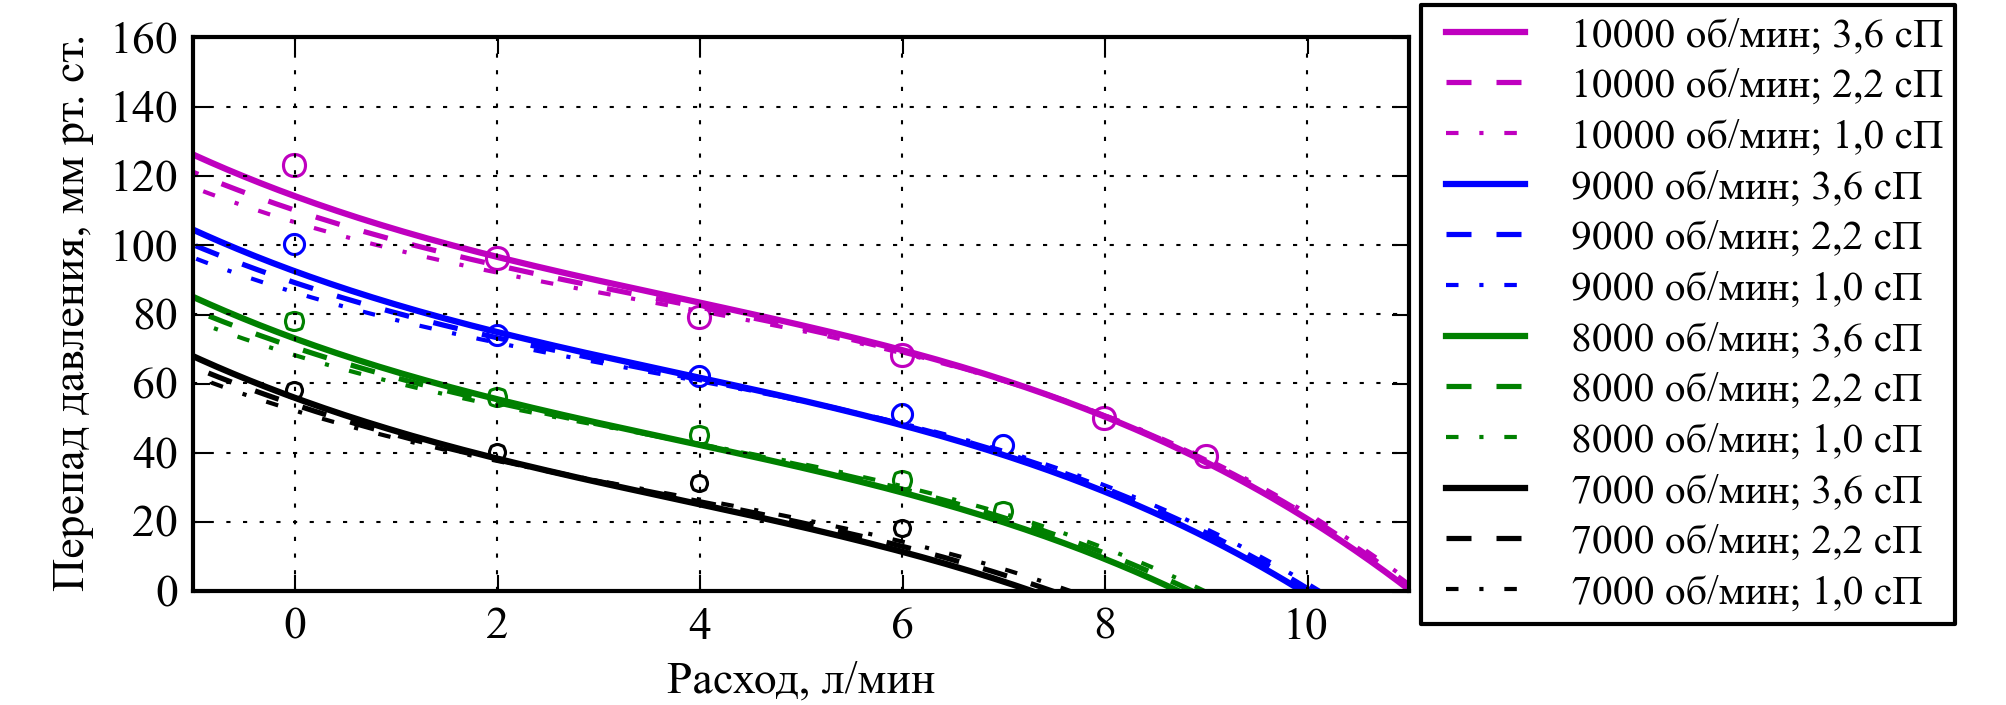
\includegraphics [scale=0.99] {../images/c2_static_model_updated_dis} \\ б)}
  \caption{Расходно-напорные характеристики роторного насоса крови, описываемые уравнением \eqref{eq:first_step_pump_model}}
  \label{img:pump_identification_second_stage}  
\end{figure}

После этого к уравнению \eqref{eq:first_step_pump_model} были добавлены члены $Q\omega^2$ и $Q^2 \omega$ вместе с поправочным коэффициентом $g = g_1\mu + g_2$, что позволило увеличить $R^2$ до 0,9987.% Полученные расходно-напорные характеристики представлены на рисунке \ref{img:pump_identification_second_stage}.

В результате было достигнуто соответствие между формой моделируемых и исходных РНХ и работа алгоритма была завершена. 

Разработанная в результате идентификации математическая модель роторного насоса крови описывается следующим уравнением: 

\begin{multline}
 L\frac{dQ}{dt} = (a_1\mu+a_2)Q + (b_1\mu+b_2)Q^2 + (c_1\mu+c_2)Q^3 + (d_1\mu+d_2)\omega^2 \\+ (e_1\mu+e_2)Q\omega^2 + (f_1\mu+f_2)Q^2\omega + g_1\mu+g_2 - H.
\label{eq:final_pump_model}
\end{multline}

Разработанная модель идентификации описывает расходно-напорные характеристики, представленные на рисунке \ref{img:final_pump_model}.

\begin{figure}[ht] 
  \center
  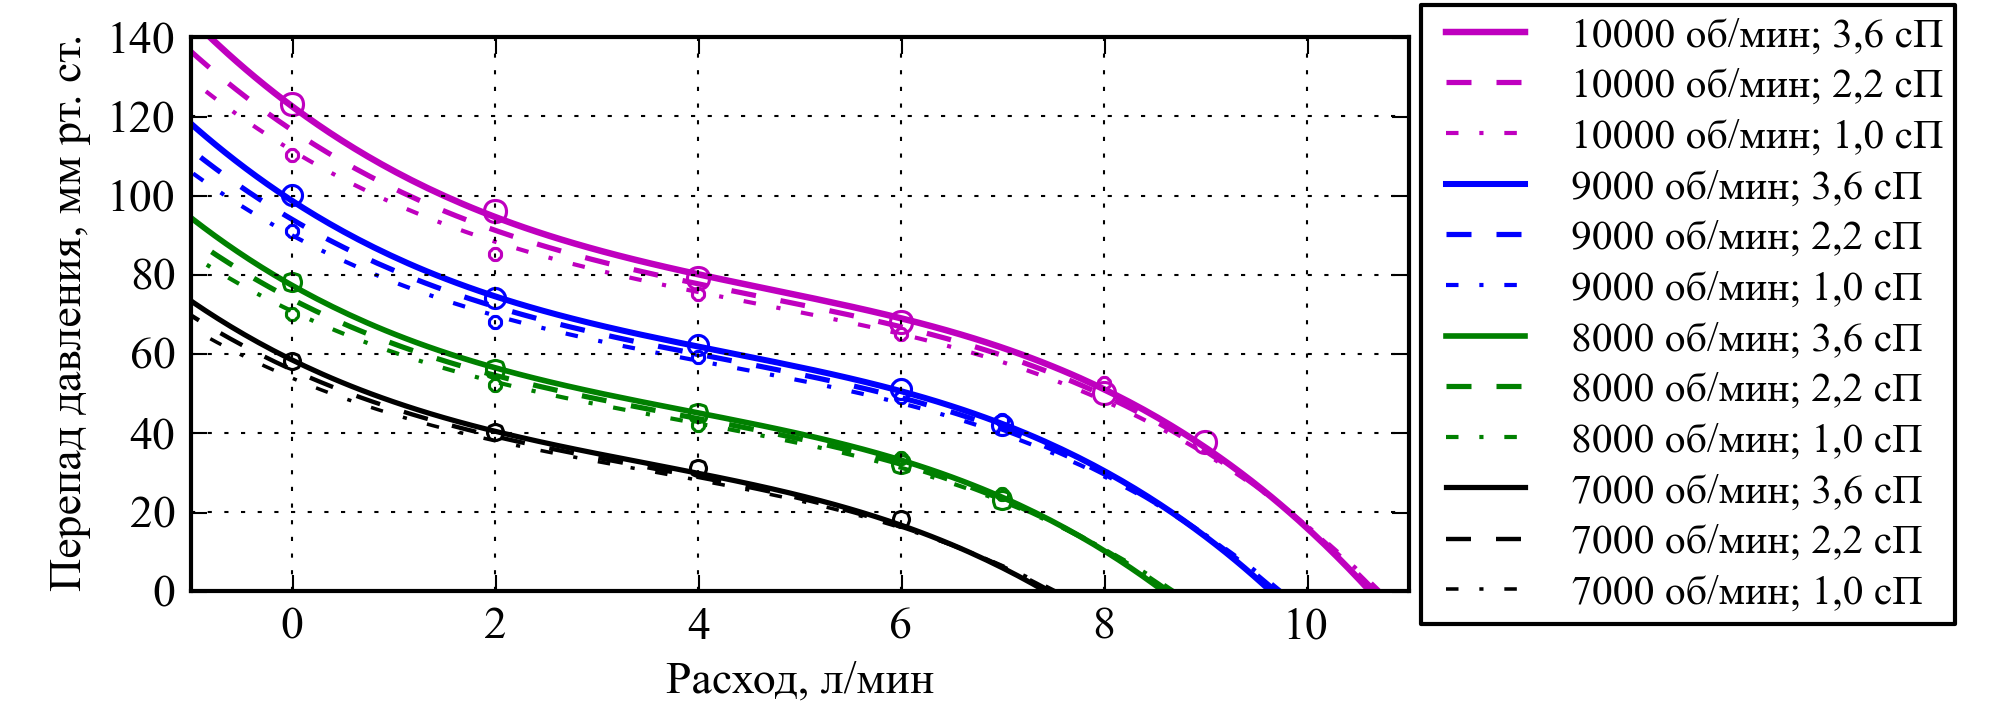
\includegraphics [scale=1.0] {../images/c2_static_model_final_dis}
  \caption{Расходно-напорные характеристики роторного насоса крови, описываемые уравнением \eqref{eq:final_pump_model}} 
  \label{img:final_pump_model}  
\end{figure}

Значения коэффициентов $a$, $b$, $c$, $d$, $e$, $f$ и $g$ приведены в таблице \ref{tbl:pump_model_coefficients}. 

\begin{table} [htbp]%
    \centering
	\caption{Коэффициенты математической модели роторного насоса крови}%
	\label{tbl:pump_model_coefficients}% label всегда желательно идти после caption
    \renewcommand{\arraystretch}{1.5} 
	\begin{tabular}{@{}@{\extracolsep{20pt}}llll@{}} 
        \toprule     %%% верхняя линейка
    	Коэффициент & Значение \\
        \midrule %%% тонкий разделитель. Отделяет названия столбцов. Обязателен по ГОСТ 2.105 пункт 4.4.5 
    	$a = a_1 + a_2\mu$ & $a_1 = -6,2332$ мм рт. ст. л$^{-1}$ \\
		 & $a_2 = -0,0254$ мм рт. ст. л$^{-1}$ сП$^{-1}$  \\
		$b = b_1 + b_2\mu$ & $b_1 = 0,5339$ мм рт. ст. л$^{-2}$  \\
		 & $b_2 = -0,0239$ мм рт. ст. л$^{-2}$ сП$^{-1}$  \\
    	$c = c_1 + c_2\mu$ & $c_1 = -0,1594$ мм рт. ст. л$^{-3}$ \\
		 & $c_2 = -0,0147$ мм рт. ст. л$^{-3}$ сП$^{-1}$  \\
		$d = d_1 + d_2\mu$ & $d_1 = 1,0778$ мм рт. ст. мин$^{2}$  \\
		 & $d_2 = 0,0495$ мм рт. ст. мин$^{2}$ сП$^{-1}$  \\
    	$e = e_1 + e_2\mu$ & $e_1 = -0,0788$ мм рт. ст. мин$^2$ л$^{-1}$ \\
		 & $e_2 = -0,0133$ мм рт. ст. мин$^2$ л$^{-1}$ сП$^{-1}$  \\
		$f = f_1 + f_2\mu$ & $f_1 = 0,1568$ мм рт. ст. мин л$^{-2}$ \\
		 & $f_2 = 0,0263$ мм рт. ст. мин л$^{-2}$ сП$^{-1}$ \\
    	$g = g_1 + g_2\mu$ & $g_1 = -0,6583$ мм рт. ст. \\
		 & $g_2 = -0,6671$ мм рт. ст. сП$^{-1}$  \\
        \bottomrule %%% нижняя линейка
	\end{tabular}%
\end{table}

Поскольку состояние РНК описывается единственной переменной $Q$, то фазовое пространство уравнения \eqref{eq:final_pump_model} одномерно и представлено вещественной прямой $0Q$. Поэтому для наглядности будем изображать эволюцию уравнения \eqref{eq:final_pump_model}, откладывая по оси абсцисс время $t$, по оси ординат -- фазовую переменную $Q$:

\begin{figure}[ht] 
  \center
  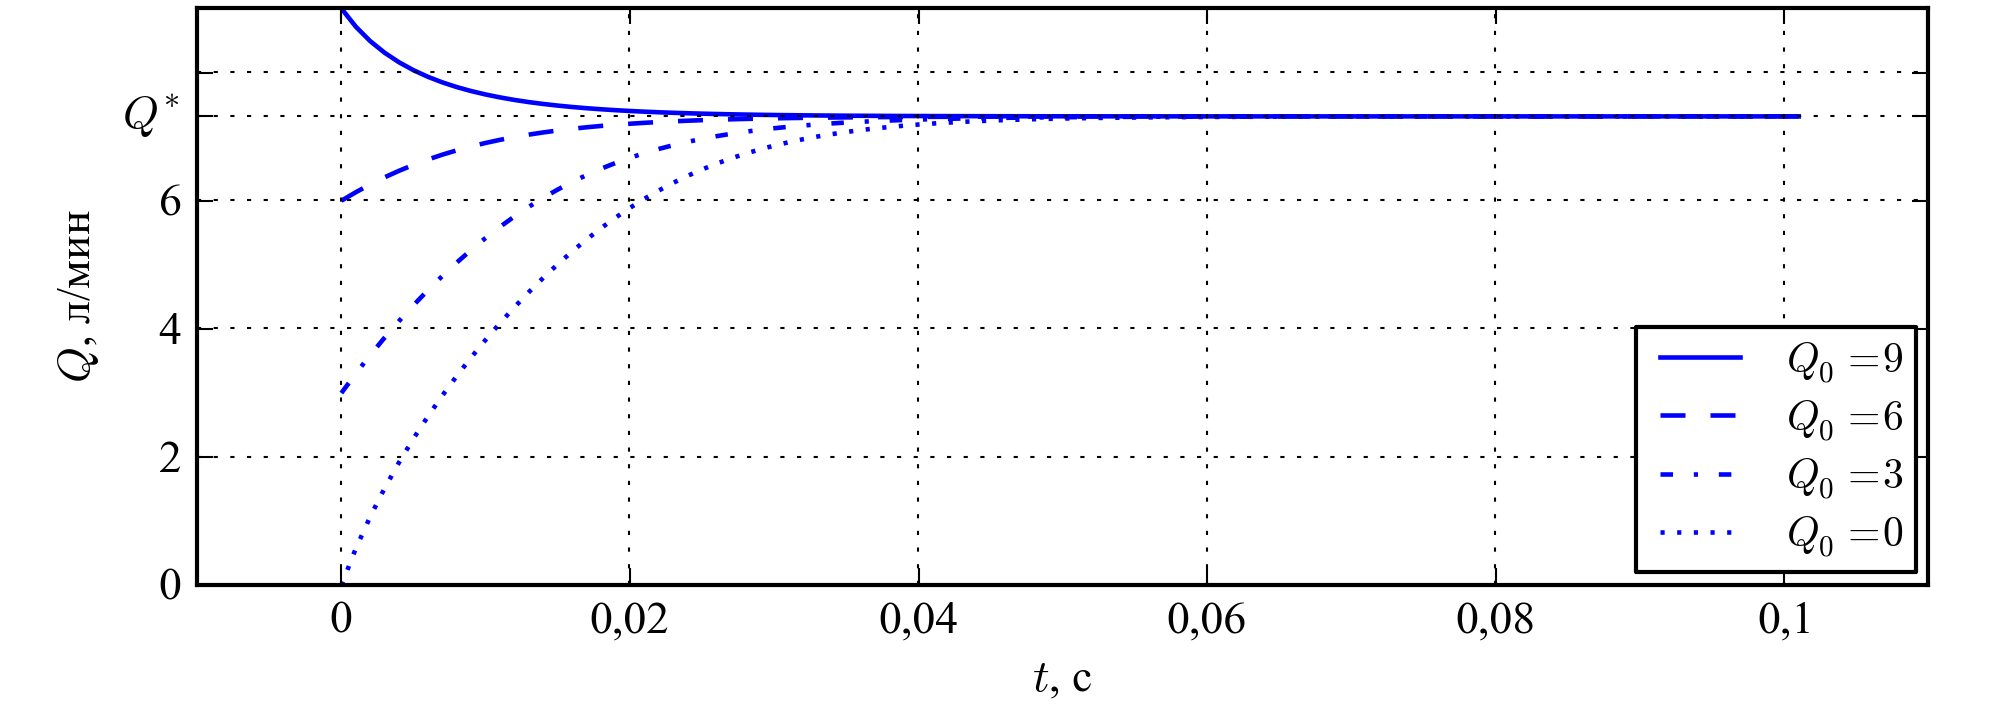
\includegraphics [scale=1.0] {../images/c2_dynamic_model_solution_zero}
  \caption{Зависимость $Q$ от времени при различных начальных условиях}
  \label{img:final_pump_model_solution_zero}  
\end{figure}

На рисунке \ref{img:final_pump_model_solution_zero} представлено изменение $Q$ от времени $t$ при различных начальных значениях $Q_0$ и фиксированных параметрах $\mu = $ 3,6 сП, $\omega =$ 8000 об/мин и $H = $ 20 мм рт. ст. Видно, что с течением времени значения переменной $Q$ стремятся к некоторому особому значению $Q^*$. При этом значения достаточно быстро выходят на $Q^*$. 

Найдем особые точки уравнения \eqref{eq:final_pump_model}, приравняв левую часть уравнения \eqref{eq:final_pump_model} к нулю:

\begin{multline}
(a_1\mu+a_2)Q + (b_1\mu+b_2)Q^2 + (c_1\mu+c_2)Q^3 + (d_1\mu+d_2)\omega^2 + \\+ (e_1\mu+e_2)Q\omega^2 + (f_1\mu+f_2)Q^2\omega + g_1\mu+g_2 - H = 0.
\label{eq:final_pump_model_zero}
\end{multline}

Уравнение \eqref{eq:final_pump_model_zero} решено с использованием формулы Кардано для нахождения корней $x_1$, $x_2$ и $x_3$ уравнения вида $ax^3 + bx^2 + cx + d = 0$:

\begin{equation}
x_1 = -\frac{b}{3a} + \alpha + \beta, \quad x_{2, 3} = -\frac{b}{3a}  - \frac{(\alpha + \beta)}{2} \pm \frac{i(\alpha - \beta)}{2}\sqrt{3},
\label{eq:cardano_1}
\end{equation}

где 

\begin{equation}
a = c_1\mu + c_2, \quad b = b_1\mu + b_2 + (f_1\mu + f_2)\omega,
\label{eq:cardano_2_1}
\end{equation}

\begin{equation}
c = a_1\mu + a_2 + (e_1\mu + e_2)\omega^2, \quad d = (d_1\mu + d_2)\omega^2 + g_1\mu + g_2 - H,
\label{eq:cardano_2_2}
\end{equation}

\begin{equation}
\alpha = \sqrt[3]{-\frac{q}{2} + \sqrt{R}}, \quad \beta = \sqrt[3]{-\frac{q}{2} - \sqrt{R}},
\label{eq:cardano_2}
\end{equation}

\begin{equation}
R = \left(\frac{p}{3}\right)^3 + \left( \frac{q}{2} \right)^2,
\label{eq:cardano_3}
\end{equation}

\begin{equation}
p = \frac{3ac - b^2}{3a^2}, \quad q = \frac{2b^3 - 9abc + 27a^2d}{27a^3}.
\label{eq:cardano_extension}
\end{equation}

По знаку $R$ можно определить тип корней. Если член $p$ больше нуля, то $R$ заведомо больше нуля и решение уравнения \eqref{eq:final_pump_model_zero} имеет один вещественный корень и два сопряженных комплексных корня. % \cite{korn1973}.

Так, в член $p$ входят параметры $\mu$ и $\omega$: параметр $\mu$ изменяется в диапазоне от 1,0 сП до 3,6 сП, параметр $\omega$ -- от 5 до 11 тысяч об/мин. На рисунке \ref{img:model_zero_roots} представлены зависимости $p$ для физически реализуемых $\mu$ и $\omega$.

\begin{figure}[ht] 
  \center
  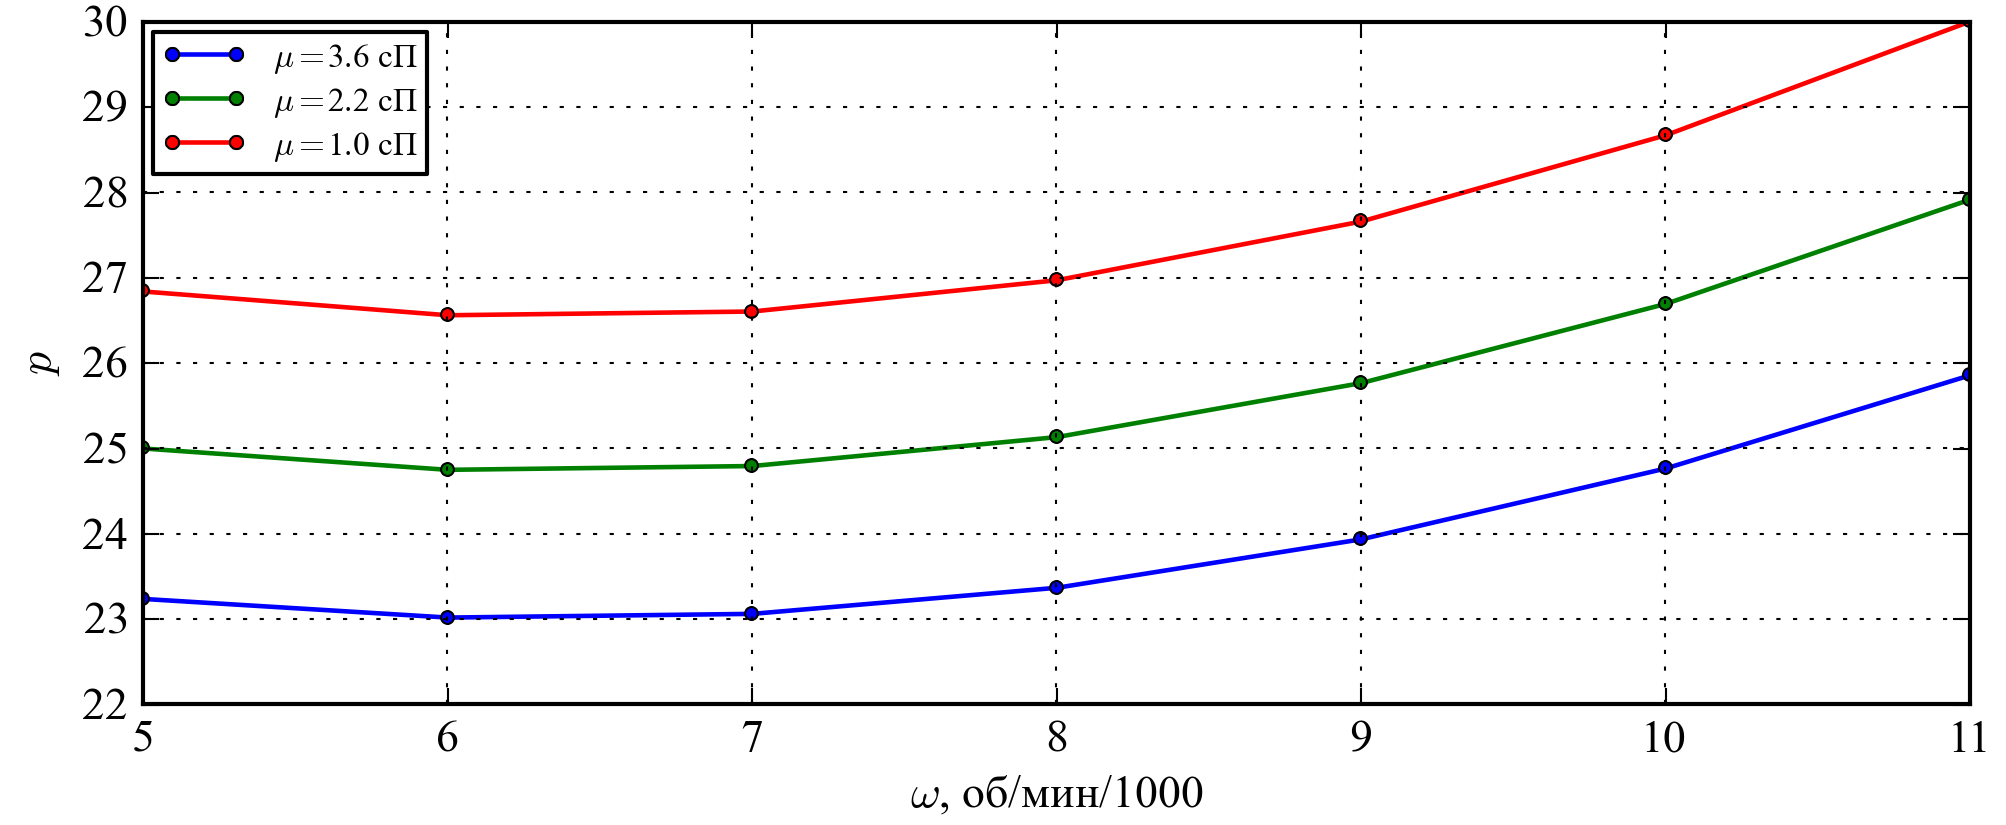
\includegraphics [scale=1.0] {../images/c2_model_zero}
  \caption{Зависимость $p$ для физических реализуемых параметров $\mu$ и $\omega$}
  \label{img:model_zero_roots}  
\end{figure}

Для уравнения \eqref{eq:final_pump_model_zero} $R > 0$, таким образом, уравнение \eqref{eq:final_pump_model_zero} имеет один вещественный корень и два сопряженных комплексных корня, следовательно, при всех физически реализуемых $\mu$, $\omega$ и $H$ особая точка уравнения \eqref{eq:final_pump_model} единственна.

%\section*{Влияние вязкости жидкости на расходно-напорную характеристику роторного насоса крови} \label{subsect2_1_1} 

% Поскольку разработанная математическая модель учитывает инерционные и вязкостные свойства крови в данной главе демонстрируется и дается количественная оценка влияния инерционных и вязкостных свойств крови на величину потока через РНК. 
% 
% Количественная оценка влияния вязкости крови на величину потока через роторный насос крови приведена на рис. \ref{img:viscosity_main} при скоростях от 5 до 9 тысяч об/мин в диапазоне вязкостей от 3,6 до 1,0 сП. Влияние изменения вязкости крови на величину потока через насоса при изменении частоты сердечных сокращений и сократимости левого желудочка сердца -- на рис. \ref{img:viscosity_HR_CV}.
% 
% \begin{figure}[ht] 
%   \center
%   \includegraphics [scale=1.0] {../images/c2_viscosity_main}
%   \caption{Влияние изменения вязкости крови $\mu$ на величину потока через насос при различных скоростях насоса} 
%   \label{img:viscosity_main}  
% \end{figure}
% 
% Видно, что уменьшение вязкости с 3,6 до 1,0 сП при фиксированной скорости приводит к уменьшению минутной расхода насоса: на 0,1 л/мин при 6000 об/мин и на 0,22 л/мин при 8000 об/мин. Таким образом, чем выше скорость насоса, тем сильнее изменение $\mu$ влияет на величину потока. Тем не менее, при 9000 об/мин влияние вязкости крови незначительно уменьшается -- до 0,09 л/мин. 
% 
% Кроме того, увеличение частоты сердечных сокращений с 60 уд/мин до 100 уд/мин также приводит к большему влиянию величины вязкости на минутный расход насоса: уменьшение $\mu$ с 3,6 до 1,0 сП при 8000 об/мин уменьшает расход на 0,25 л/мин. Влияние сократимости левого желудочка сердца аналогично ЧСС: увеличение параметра $C_V$ на 10\% приводит к усилению вязкости крови на расход насоса.
% 
% \begin{figure}[ht] 
%   \center
%   \includegraphics [scale=1.0] {../images/c2_viscosity_HR_CV}
%   \caption{Влияние изменения вязкости крови $\mu$ на величину потока через насос при различных скоростях насоса и изменении частоты сердечных сокращений (ЧСС, уд/мин) и сократимости левого желудочка сердца ($C_V$, \%)} 
%   \label{img:viscosity_HR_CV}  
% \end{figure}
% 
% Таким образом, усиление сердечной функции, независимо от того обусловлено ли оно увеличением ЧСС или сократимости ЛЖ, приводит к увеличению влияния вязкости крови на минутный расход насоса.  
% 
% Количественная оценка влияния параметра $L$ на величину потока через роторный насос крови приведена на рис. \ref{img:inertia_main} при скоростях от 5 до 9 тысяч об/мин в диапазоне параметра $L$ от 0.2 до 0.8. Влияние изменения $L$ на величину потока через насоса при изменении частоты сердечных сокращений и сократимости левого желудочка сердца -- на рис. \ref{img:inertia_HR_CV}.
% 
% \begin{figure}[ht] 
%   \center
%   \includegraphics [scale=1.0] {../images/c2_inertia_main}
%   \caption{Влияние изменения параметра $L$ на величину потока через насос при различных скоростях насоса} 
%   \label{img:inertia_main}  
% \end{figure}
% 
% \begin{figure}[ht] 
%   \center
%   \includegraphics [scale=1.0] {../images/c2_inertia_HR_CV}
%   \caption{Влияние изменения параметра $L$ на величину потока через насос при различных скоростях насоса и изменении частоты сердечных сокращений (ЧСС, уд/мин) и сократимости левого желудочка сердца ($C_V$, \%)} 
%   \label{img:inertia_HR_CV}  
% \end{figure}
% 
% Видно, что увеличение параметра $L$ до 0,8 приводит к уменьшению минутного расхода насоса в диапазоне скоростей от 5000 до 8000 об/мин. В то же время, его влияние уменьшается с увеличением скорости насоса до 9000 об/мин, при этом увеличение $L$ приводит к незначительному увеличению расхода на 0,04 л/мин.
% 
% Увеличение частоты сердечных сокращений и сократимости ЛЖ также приводит к увеличению влияния параметра $L$. В этом случае при ЧСС 100 уд/мин и скорости 6000 об/мин увеличение $L$ до 0.8 уменьшает расхода насоса на 0,32 л/мин. Аналогичным образом, влияние параметра $L$ уменьшается с увеличением скорости насоса и минимальное изменение минутного расхода при увеличении $L$ до 0,8 составляет 0,08 л/мин (скорость 8000 об/мин и ЧСС 60 уд/мин).
% 
% На рис. \ref{img:L_mu_influence} продемонстрировано влияние вязкости крови при различных величинах параметра $L$. Во всех случаях уменьшение вязкости крови до 1,0 сП приводит к уменьшению минутного расхода насоса; при этом увеличение скорости также усиливает влияние вязкостных свойств крови на минутный расхода насоса аналогично рис. \ref{img:viscosity_main}. В то же время, увеличение $L$ с 0.2 до 0.8 приводит к увеличению влияния вязкостных свойств крови. Самое малое изменение в расходе насоса на 0,15 л/мин происходит при уменьшении вязкости с 3,6 до 1,0 сП, скорости 6000 об/мин и $L$ = 0.2.
% 
% \begin{figure}[ht] 
%   \center
%   \includegraphics [scale=1.0] {../images/c2_L_mu_influence}
%   \caption{Влияние изменения вязкости крови $\mu$ на величину потока через насос при различных величинах скорости насоса и параметра $L$} 
%   \label{img:L_mu_influence}  
% \end{figure}
% 
% В данной главе также предлагается алгоритм управления расходом роторного насоса крови. Разработанная математическая модель РНК позволяет оценивать только мгновенный расход, поэтому реализация метода оценки потока в системе управления предполагает реализацию алгоритма управления расходом насоса. 
% 
% Структурная схема алгоритма управления расходом РНК показана на рис. \ref{img:simple_control_algorithm}. Она состоит из трех блоков. Основным компонентом блока РНК является математическая модель РНК, которая позволяет оценить поток в данный момент времени на основе значений скорости $\omega$, перепада давления $H$ и вязкости крови $\mu$, величина которой задается на внешней консоли управления.
% 
% В оценочном блоке производится оценка минутного ($Q_P$) и приближенного ($Q_A$) расходов РНК на основе временной диаграммы расхода, сформированной благодаря блоку РНК.   
% 
% \begin{figure}[ht] 
%   \center
%   \includegraphics [scale=1.7] {../images/c2_simple_control_algorithm}
%   \caption{Структурная схема алгоритма управления расходом роторного насоса крови}
%   \label{img:simple_control_algorithm}
% \end{figure}
% 
% На рис. \ref{img:flow_estimation} показаны два способа оценки минутного и приближенного расходов. В первом случае используется временная диаграмма расхода на временном промежутке в 60 секунд; интегрирование расходной характеристики в указанном диапазоне позволяет определить минутный расход насоса $Q_P$ (л/мин).
% 
% \begin{figure}[ht] 
%   \center
%   \includegraphics [scale=1.0] {../images/c2_flow_estimation}
%   \caption{Оценка (А) минутного расхода насоса ($Q_P$, л/мин) и (Б) приближенного расхода ($Q_A$, л/мин) по временной диаграмме расхода насоса (л/с)}
%   \label{img:flow_estimation}
% \end{figure}
% 
% Во втором случае на временной диаграмме находится минимум, который соответствует началу диастолической фазы сердечного цикла. Следующий минимум обозначает окончание данного сердечного цикла и начало новой диастолической фазы. Таким образом, можно определить промежуток времени, соответствующий определенному количеству сердечных циклов (в данном случае пяти). Из этих данных можно найти частоту сердечных сокращений и объем крови, который перекачан насосом за это время. Полученное значение аппроксимируется до литров в минуту и считается приближенным расходом насоса. 
% 
% В блоке регулировки скорости производится сравнение приближенного и требуемого уровня расхода $Q_D$, которое задается на внешней консоли управления. При их несовпадении происходит изменение скорости РНК на 100 об/мин.  
% 
% Пример использования данного способа оценки расхода с целью регулировки расхода насоса относительно требуемого значения при изменении физиологических условий показан на рис. \ref{img:estimated_flow_variation}. В этом случае изменение частоты сердечных сокращений от 60 уд/мин до 100 уд/мин при $Q_D =$ 3,8 л/мин приводит к соответствующими изменениями скорости РНК. 
% 
% \begin{figure}[ht] 
%   \center
%   \includegraphics [scale=1.0] {../images/c2_estimated_flow_variation}
%   \caption{Временная диаграмма изменения расхода ($Q_P$ и $Q_A$, л/мин), скорости насоса ($\omega_P$, об/мин/1000) и частоты сердечных сокращений (ЧСС, уд/мин)}
%   \label{img:estimated_flow_variation}
% \end{figure}
% 
% Видно, что уменьшение ЧСС до 60 уд/мин сопровождается уменьшением приближенного расхода относительно желаемого значения $Q_D$, поэтому скорость насоса начинает увеличиваться. Использование приближенного расхода $Q_A$ и его периодическое сравнение с $Q_D$ позволяет довольно быстро реагировать на физиологические изменения, такие как изменение ЧСС, и поддерживать расход РНК $Q_P$ на требуемом уровне.  

\section{Математические модели сердечной-сосудистой системы} \label{cvs_model_implementation}

В данной части приводится описание разработки математической модели сердечно-сосудистой системы с использованием математических моделей сердца и системы кровообращения.

\subsection*{Математическая модель системы кровообращения}

Система кровообращения описана математическими моделями с сосредоточенными параметрами на основе аналогии между течением крови в артерии и током в электрической цепи \cite{Kokalari_2013, shi2011review}. Пример такой аналогии представлен на рисунке \ref{img:blood_current_analogy}. Градиент давлений перемещает кровь из левого желудочка (ЛЖ) в аорту, преодолевая гидравлическое сопротивление так же, как и градиент напряжения в электрической цепи заставляет ток течь, преодолевая электрическое сопротивление. Таким образом, описывая давление и течение крови с помощью напряжения и тока, а эффекты трения, инерции крови и эластичность сосуда с помощью сопротивления $R$, индуктивности $L$ и емкости $C$ соответственно, можно использовать известные методы анализа электрических цепей для исследования кровообращения в сердечно-сосудистой системе. 

\begin{figure}[ht] 
  \center
  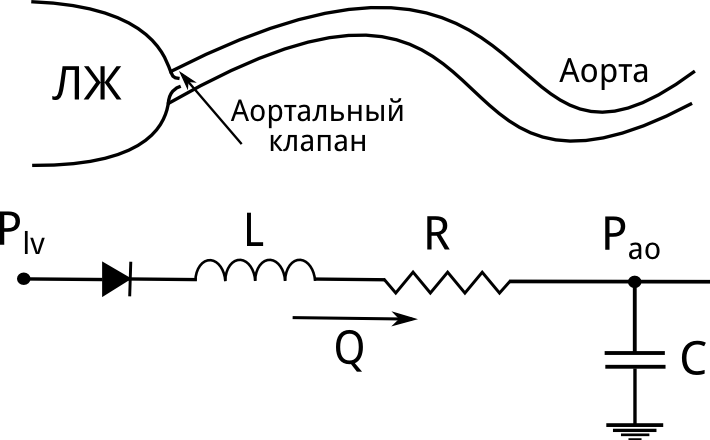
\includegraphics [scale=1.1] {../images/c2_electric_analogy}
  \caption{Пример аналогии между течением крови в аорте и током в электрической цепи; $P_{lv}$ -- давление в левом желудочке сердца, $P_{ao}$ -- давление в аорте, $L$ -- индуктивность, $R$ -- сопротивление, $C$ -- емкость, $Q$ -- поток}
  \label{img:blood_current_analogy}
\end{figure}

Математическая модель системы кровообращения представлена на рисунке \ref{img:full_cvs} в виде электрически-эквивалентной схемы аналогично работам \cite{Cox_2009, Martina_2013_simulation}. 

\begin{figure}[htb]
	\center{
\includegraphics[width=1.0\linewidth]{../images/c2_cvs}}
	\caption{Математическая модель сердечно-сосудистой системы, представленная в виде электрически-эквивалентной схемы}
	\label{img:full_cvs}
\end{figure}

Большой и малый круги кровообращения составлены из артериального, периферического и венозного сосудистых сегментов. Каждый сегмент моделируется с помощью постоянных сопротивлений $R$, индуктивностей $L$ и емкостей $C$. Падение давления на каждом из этих элементов описывается следующими уравнениями:

\begin{equation}
\begin{aligned}
\Delta P_R &= RQ, & \Delta P_L &= L\frac{dQ}{dt}, & \Delta P_C &= \frac{V-V_0}{C},
\end{aligned}
\end{equation}

\noindent где $Q$ -- поток через элемент, $V$ -- объем и $V_0$ -- объем при нулевом давлении. 

Исходные величины элементов электрической цепи были взяты из работ \cite{Cox_2009, Martina_2013_simulation}.  % добавить таблицу?

Скорость изменения объема в каждом сегменте вычисляется следующим образом \cite{smith2005experimentally}:

\begin{equation}
	\frac{ dV }{dt} =Q_{in} - Q_{out},
\end{equation}

Артериальные участки большого и малого кругов кровообращения составлены из $n$ сегментов, где $n$ в данном случае равняется пяти. Это позволяет моделировать постепенное уменьшение пульсаций в артерии и подключение выхода насоса к различным участкам артерии. Обозначения \verb!art_L! и \verb!art_R! соответствуют артериальным сегментам большого и малого круга, \verb!ven_L! и \verb!ven_R! -- венозным сегментам большого и малого кругов кровообращения; номера рядом с ними определяют номер сегмента. Обозначение \verb!R_p! соответствует сопротивлению периферического кровообращения, \verb!Plv! и \verb!Prv! -- давлениям в левом и правом желудочках сердца, \verb!Rav!, \verb!Rtr!, \verb!Rpv!, \verb!Rmv! -- сопротивлениям аортального, трикуспидного, пульмонального и митрального клапанов сердца, \verb!Pcv! и \verb!Ppcw! -- центральному венозному давлению и давлению заклинивания в легочных капиллярах.

Скорость изменения потока в сегментах с индуктивностью определяется разностью давлений $P$, сопротивлением между ними $R$ и величиной индуктивности $L$ \cite{smith2005experimentally}:

\begin{equation}
	\frac{ dQ }{dt} = \frac{ P_{lv} - P_{ao} - Q(R_{valve} + R) }{ L },
\end{equation}

Течение крови в периферических сегментах, содержащих только сопротивление $R$, описывается законом Ома для участка цепи:

\begin{equation}
	\frac{ dQ }{dt} = \frac{ P_{art} - P_{ven} }{ R_{p} },
\end{equation}

\subsection*{Математическая модель сердца}

На рисунке \ref{img:full_cvs} сердце представлено левым (lv) и правым (rv) желудочками, включая клапаны сердца: митральный (mv), аортальный (av), трехстворчатый (tv) и легочный (pv). Поведение клапана моделируется с помощью идеальных диодов с постоянным высоким сопротивлением при обратном течении ($Q_{valve} \leq 0$) и постоянным низким сопротивлением при прямом течении ($Q_{valve} > 0$) через клапан:

\begin{equation}
	R_{valve} =  \begin{cases} 10^{12}, & Q_{valve} \leq 0 \\ 1, & Q_{valve} > 0 \\ \end{cases} 
\end{equation}

\noindent где $R_{valve}$ -- сопротивление клапана, $Q_{valve}$ -- поток через клапан. 

Работа желудочков сердца описывается моделью <<единичного волокна>>, которая связывает макроскопические параметры, такие как давление и объем, с микроскопическими свойствами сердечной ткани -- сократительная способность миокарда, длина саркомеры. Математическая модель первоначально была представлена в работе T. Arts и др. \cite{Arts_1991} и впоследствии адаптирована в работах \cite{Arts2003731, Bovendeerd_2006}. %предполагает пространственную однородность натяжения и напряжения сердечного волокна, . 
 
Основное уравнения, позволяющее определить давление в желудочке $P_v$ по величине объема $V_v$, записывается в следующем виде:

\begin{equation}
	\label{eq:heart}
	P_v = \frac{1}{3} (\sigma_f - 2 \sigma_{m,r}) \ln \left(1 + \frac{V_w}{V_v}\right),
\end{equation}

\noindent где $P_v$ -- давление в желудочке, $V_w$ -- объем стенки желудочка, $V_v$ -- объем камеры желудочка, $\sigma_{m,r}$ -- поперечное радиальное натяжение. 

Уравнение для суммарного натяжения $\sigma_f$ записывается следующим образом:

\begin{equation}
	\sigma_f = \sigma_a + \sigma_{m,f},
\end{equation}

\noindent где $\sigma_{m,f}$ -- пассивное натяжение вдоль волокон сердечной мышцы, $\sigma_a$ -- действительное натяжение, определяемое следующим выражением:

\begin{equation}
	\sigma_a = C_V \sigma_{ar} f(l_s) g(t_a) h(\nu_s),
\end{equation}

\noindent где $C_V$ -- параметр, характеризующий сократительную способность и определяющий долю натяжения, индуцируемого миокардом во время сокращения волокон, $\sigma_{ar}$ -- исходное значения натяжения волокна. 

Значения $\sigma_{m,f}$ и $\sigma_{m,r}$ определяются следующим образом:

\begin{equation}
	\sigma_{m,f} = \begin{cases} \sigma_{f0} \left(e^{S_f (\lambda_f -1)} -1 \right), &\lambda_f \geq 1 \\ 0, &\lambda_f < 1 \\ \end{cases}
\end{equation}

\begin{equation}
	\sigma_{m,r} = \begin{cases} \sigma_{r0} \left(e^{S_r (\lambda_r -1)} -1 \right), &\lambda_r \geq 1 \\ 0, &\lambda_r < 1 \\ \end{cases}
\end{equation}

\noindent где $\lambda_f$ -- степень растяжения волокна, $\lambda_r$ -- степень растяжения в радиальном направлении, $S_f$ и $S_r$ определяют степень прогрессивности пассивного натяжения по отношению к напряжению.

Значения $\lambda_f$ и $\lambda_r$ определяются следующими выражениями:

\begin{gather*}
  \lambda_f = \left\{\frac{V_v + \frac{1}{3} V_w}{V_{v0} + \frac{1}{3} V_w} \right\}, \\
  \lambda_r = \lambda_f ^{-2},
\end{gather*}

\noindent где $V_{v0}$ -- объем желудочка при нулевом давлении в камере желудочка. 

\begin{equation}
	f(l_s) =  \begin{cases} 0, & l_s \leq l_{s,a0} \\ \frac{l_s - l_{s,a0}}{l_{s,ar} - l_{s,a0}}, & l_s > l_{s,a0} \\ \end{cases}
\end{equation}

\noindent где $f(l_s)$ определяет натяжение волокна относительно длины саркомеры, $l_{s,a0}$ -- длина саркомеры, ниже которой действительное натяжение становится равным нулю, $l_{s,ar}$ -- длина саркомеры, которой соответствует величина исходного натяжения $\sigma_{ar}$.

\begin{equation}
	g(t_a) = \begin{cases} 0, &t_a < 0 \\ \sin^2 \left(\pi \frac{t_a}{t_{max}} \right), &0 \leq t_a \leq t_{max} \\ 0, &t_a > t_{max} \\  \end{cases}
\end{equation}

\noindent где $g(t_a)$ -- описывает активацию (начало) сокращения сердечного волокна во времени, где $t_a$ и $t_{max}$ соответствуют времени прошедшем с начала активации и продолжительности сокращения миокарда. 

\begin{equation}
	h(\nu_s) = \frac{1 - \nu_s \/ \nu_0}{1 + c_\nu (\nu_s \/ \nu_0)},
\end{equation}

\noindent где $h(\nu_s)$ -- гиперболическая функция, описывающая влияние скорости сокращения саркомеры $\nu_s$, $\nu_0$ -- исходная скорость сокращения, параметр $c_v$ определяет форму зависимости натяжения от скорости. 

\subsection{Результаты моделирования}

Разработанная математическая модель позволяет описать гемодинамику в сердечно-сосудистой системе -- динамику движения крови по сосудам. 

С целью описания гемодинамики в случае сердечной недостаточности из литературных данных были взяты гемодинамические показатели, характерные для сердечной недостаточности -- таблица \ref{tbl:cvs_model_reference_comparison} \cite{Cox_2009, Martina_2013_simulation}. 

Параметры математической модели были определены с использованием разработанной процедуры оптимизации на основе алгоритма Левенберга-Марквардта таким образом, чтобы математическая модель обеспечила соответствовала требуемым показателям гемодинамики -- столбец <<Данные>> в таблице \ref{tbl:cvs_model_reference_comparison}. В результате оптимизации математическая модель сердечно-сосудистой системы позволила описать гемодинамику в сердечно-сосудистой системе в случае сердечной недостаточности согласно работам \cite{Cox_2009, Martina_2013_simulation}. 

\begin{table} [htbp]%
    \centering
	\caption{Показатели гемодинамики, полученные на модели сердечно-сосудистой системы и из литературных данных}%
	\label{tbl:cvs_model_reference_comparison}
    \renewcommand{\arraystretch}{1.5} 
	\begin{tabular}{@{}@{\extracolsep{20pt}}llll@{}} 
        \toprule     %%% верхняя линейка
    	Показатель гемодинамики \\(единицы измерения)	& Модель  & Данные \\
        \midrule %%% тонкий разделитель. Отделяет названия столбцов. Обязателен по ГОСТ 2.105 пункт 4.4.5 
    	Систолическое артериальное давление \\(мм рт. ст.) & 82,70 & 83 \\
    	Диастолическое артериальное давление \\(мм рт. ст.) & 55,04 	 & 55	 \\
    	Систолическое давление в \\ легочной артерии (мм рт. ст.)	& 33,99 	 & 34 \\
		Диастолическое давление в \\легочной артерии (мм рт. ст.)	& 18,99 	 & 19 \\
		Центральное венозное давление \\(мм рт. ст.)	& 1,24 & 1,25 \\
		Давление заклинивания в \\легочных капиллярах (мм рт. ст.)	& 16,90 	 & 16,90 \\
		Конечно-систолический объем (мл)	& 214,94 	 & 215 \\
		Конечно-диастолический объем (мл)	& 258,93 	 & 259 \\
		Ударный объем (мл)	& 43,99 & 44 \\
        \bottomrule 
	\end{tabular}%
\end{table}

На рисунке \ref{img:cvs_hemodynamics} представлена гемодинамика в сердечно-сосудистой системе в случае сердечной недостаточности, описываемая разработанной математической моделью при частоте сердечных сокращений 80 уд/мин.

\begin{figure}[ht] 
  \center
  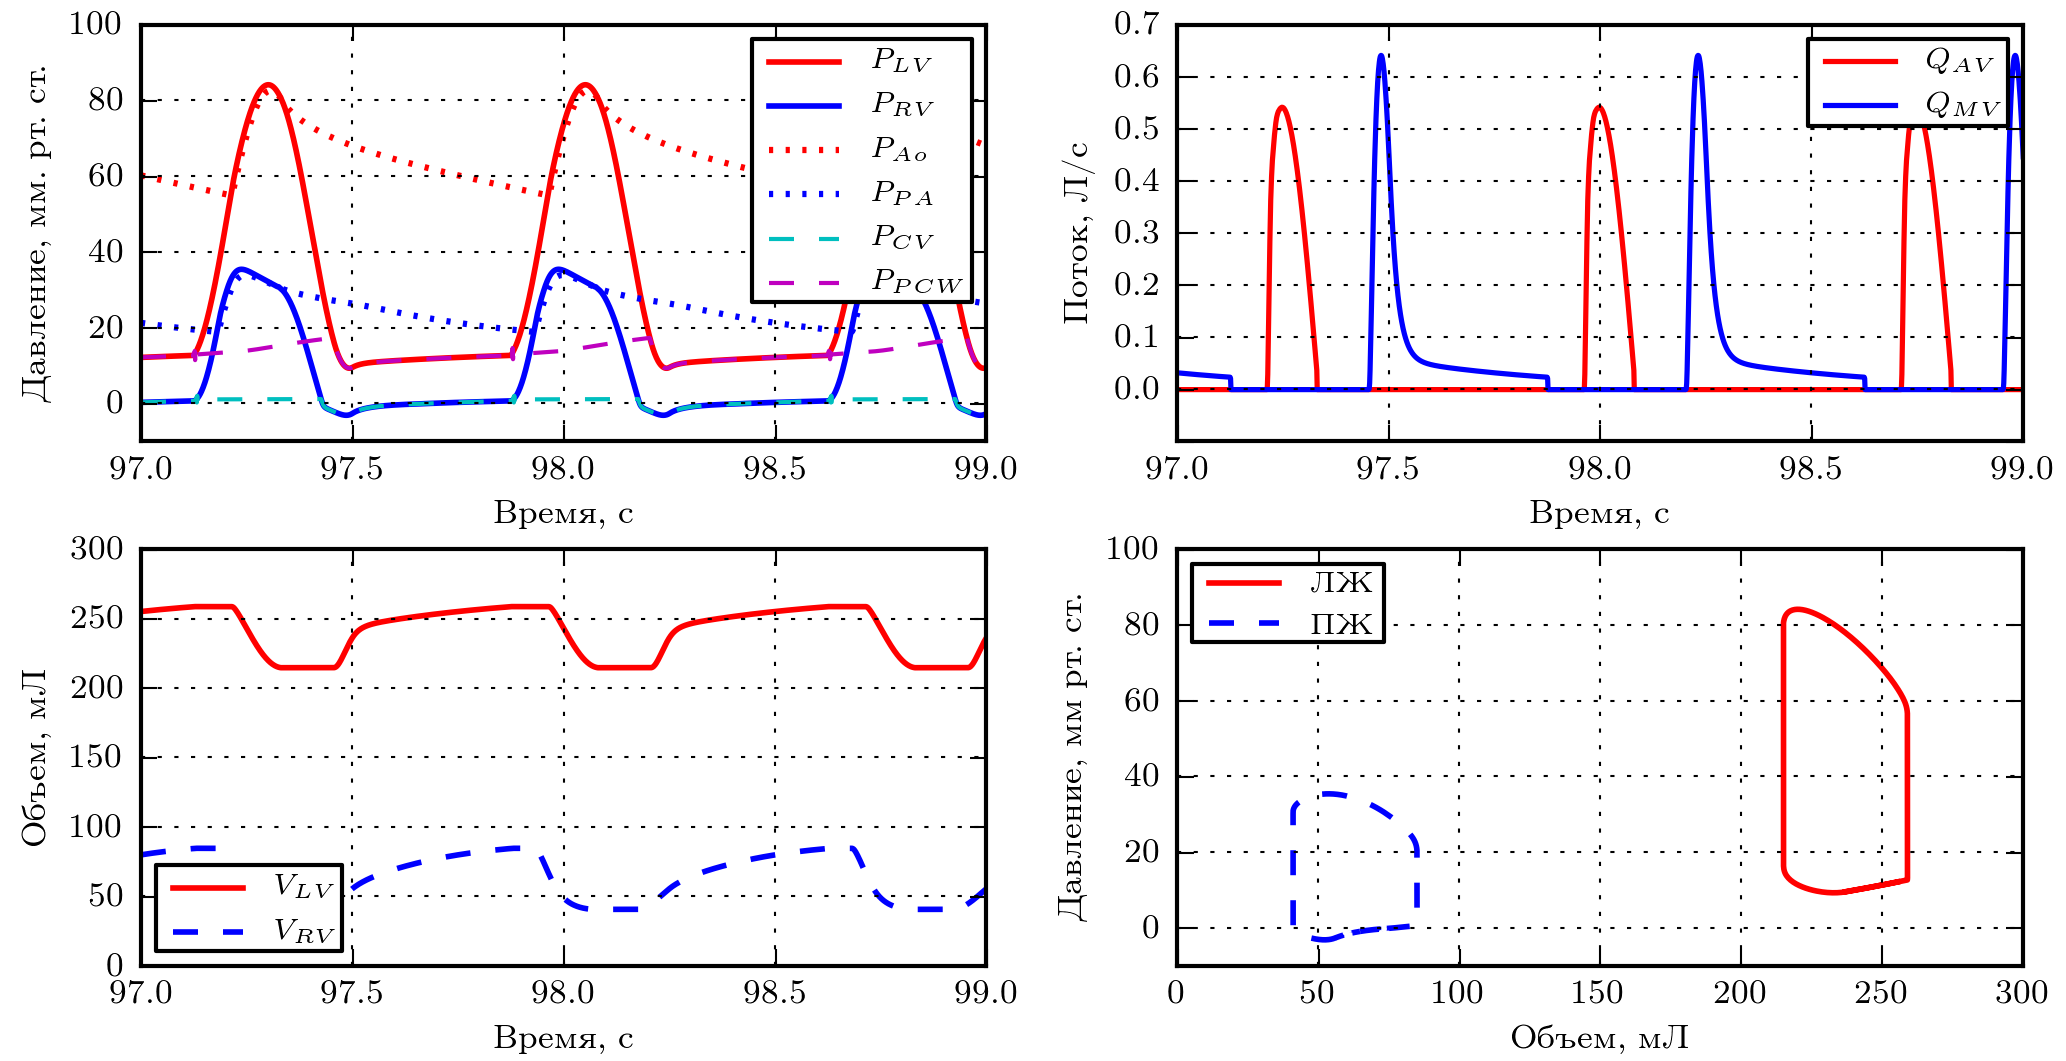
\includegraphics [scale=1.0] {../images/c2_cvs_hemodynamics}
  \caption{Гемодинамика в сердечно-сосудистой системе для случая сердечной недостаточности; $P_{LV}$ -- давление в левом желудочке сердца, $P_{RV}$ -- давление в правом желудочке сердца, $P_{Ao}$ -- давление в аорте, $P_{PA}$ -- давление в легочной артерии, $P_{CV}$ -- центральное венозное давление, $P_{PCW}$ -- давление заклинивания в легочных капиллярах, $V_{LV}$ и $V_{RV}$ -- объемы левого и правого желудочков сердца, $Q_{AV}$ и $Q_{MV}$ -- потоки через аортальный и митральный клапаны}
  \label{img:cvs_hemodynamics}
\end{figure}

Представленная гемодинамика характеризуется большим объемом левого желудочка сердца, а также меньшим систолическим давлением в аорте по сравнению с гемодинамикой в нормально функционирующей сердечно-сосудистой системе. Сдвиг контура давление-объем для левого желудочка сердца вправо вместе с уменьшением его площади согласуется с комбинированным типом сердечной недостаточности, описанным в разделе \ref{chapt1_history}.

% Рассмотренное состояние используется далее при исследовании взаимодействия насоса и сердечно-сосудистой системы.

Результаты разработки математической модели сердечно-сосудистой системы были представлены на 21-й Всероссийской конференции <<Микроэлектроника и информатика>> \cite{miee_2014}.

Разработанная математическая модель характеризуется широкими возможностями для модификации. Так, на основе рассмотренной математической модели разработаны модель сердечно-сосудистой системы педиатрических пациентов с врожденными пороками сердца \cite{mt4_2016} и модель сердечно-сосудистой системы для исследования механической поддержки кровообращения обоих желудочков сердца \cite{rgc_2016}.

Разработанная математическая модель реализована на языке программирования Python с использованием библиотеки NumPy. Программный код приведен в приложении \ref{list:cardiovascular_system_model}. 

\section*{Выводы по главе 2} 
\addcontentsline{toc}{section}{Выводы по главе 2}

В данной главе разработан алгоритм структурно-параметрической идентификации, который позволил построить математическую модель насоса на основе расходно-напорных характеристик роторного насоса крови HeartMate II. 

В ходе разработки модели идентификации реализована процедура оптимизации на основе алгоритма Левенберга-Марквардта, которая используется для определения коэффициентов математических моделей. 

Построенная в результате идентификации математическая модель имплантируемого роторного насоса крови позволяет оценивать расход насоса на основе данных о скорости вращения ротора, перепаде давления в насосе и вязкости жидкости в насосе.

В данной главе также разработана математическая модель сердечно-сосудистой системы с учетом имплантации роторного насоса крови. Разработанная математическая модель позволяет описать гемодинамику в сердечно-сосудистой системе в случае сердечной недостаточности. 
